\section{Tests préliminaires \label{aimant}}
Le but des tests préliminaires est de vérifier que les analyses effectuées dans la phase de recherche sont applicables et si la mise en
place du système imaginé lors de la phase de sélection du matériel est aussi efficace qu'espéré.

Il a été envisagé de contrôler la télécommande via un système de préhenseur d'aimant de levage. Les données disponibles de la télécommande
ne stipule pas la force nécessaire à l'activation d'un de ses boutons.

Le préhenseur a été installé sur une pièce imprimée en 3D permettant d'actionner la télécommande sans avoir d'effet de recul.
La hauteur est déterminée de manière à pouvoir glisser la télécommande entre les plaques tout en garantissant que la tige puisse se déployer sur
une longueur suffisante pour atteindre son pic de force.

\begin{figure}[H]
    \centering
    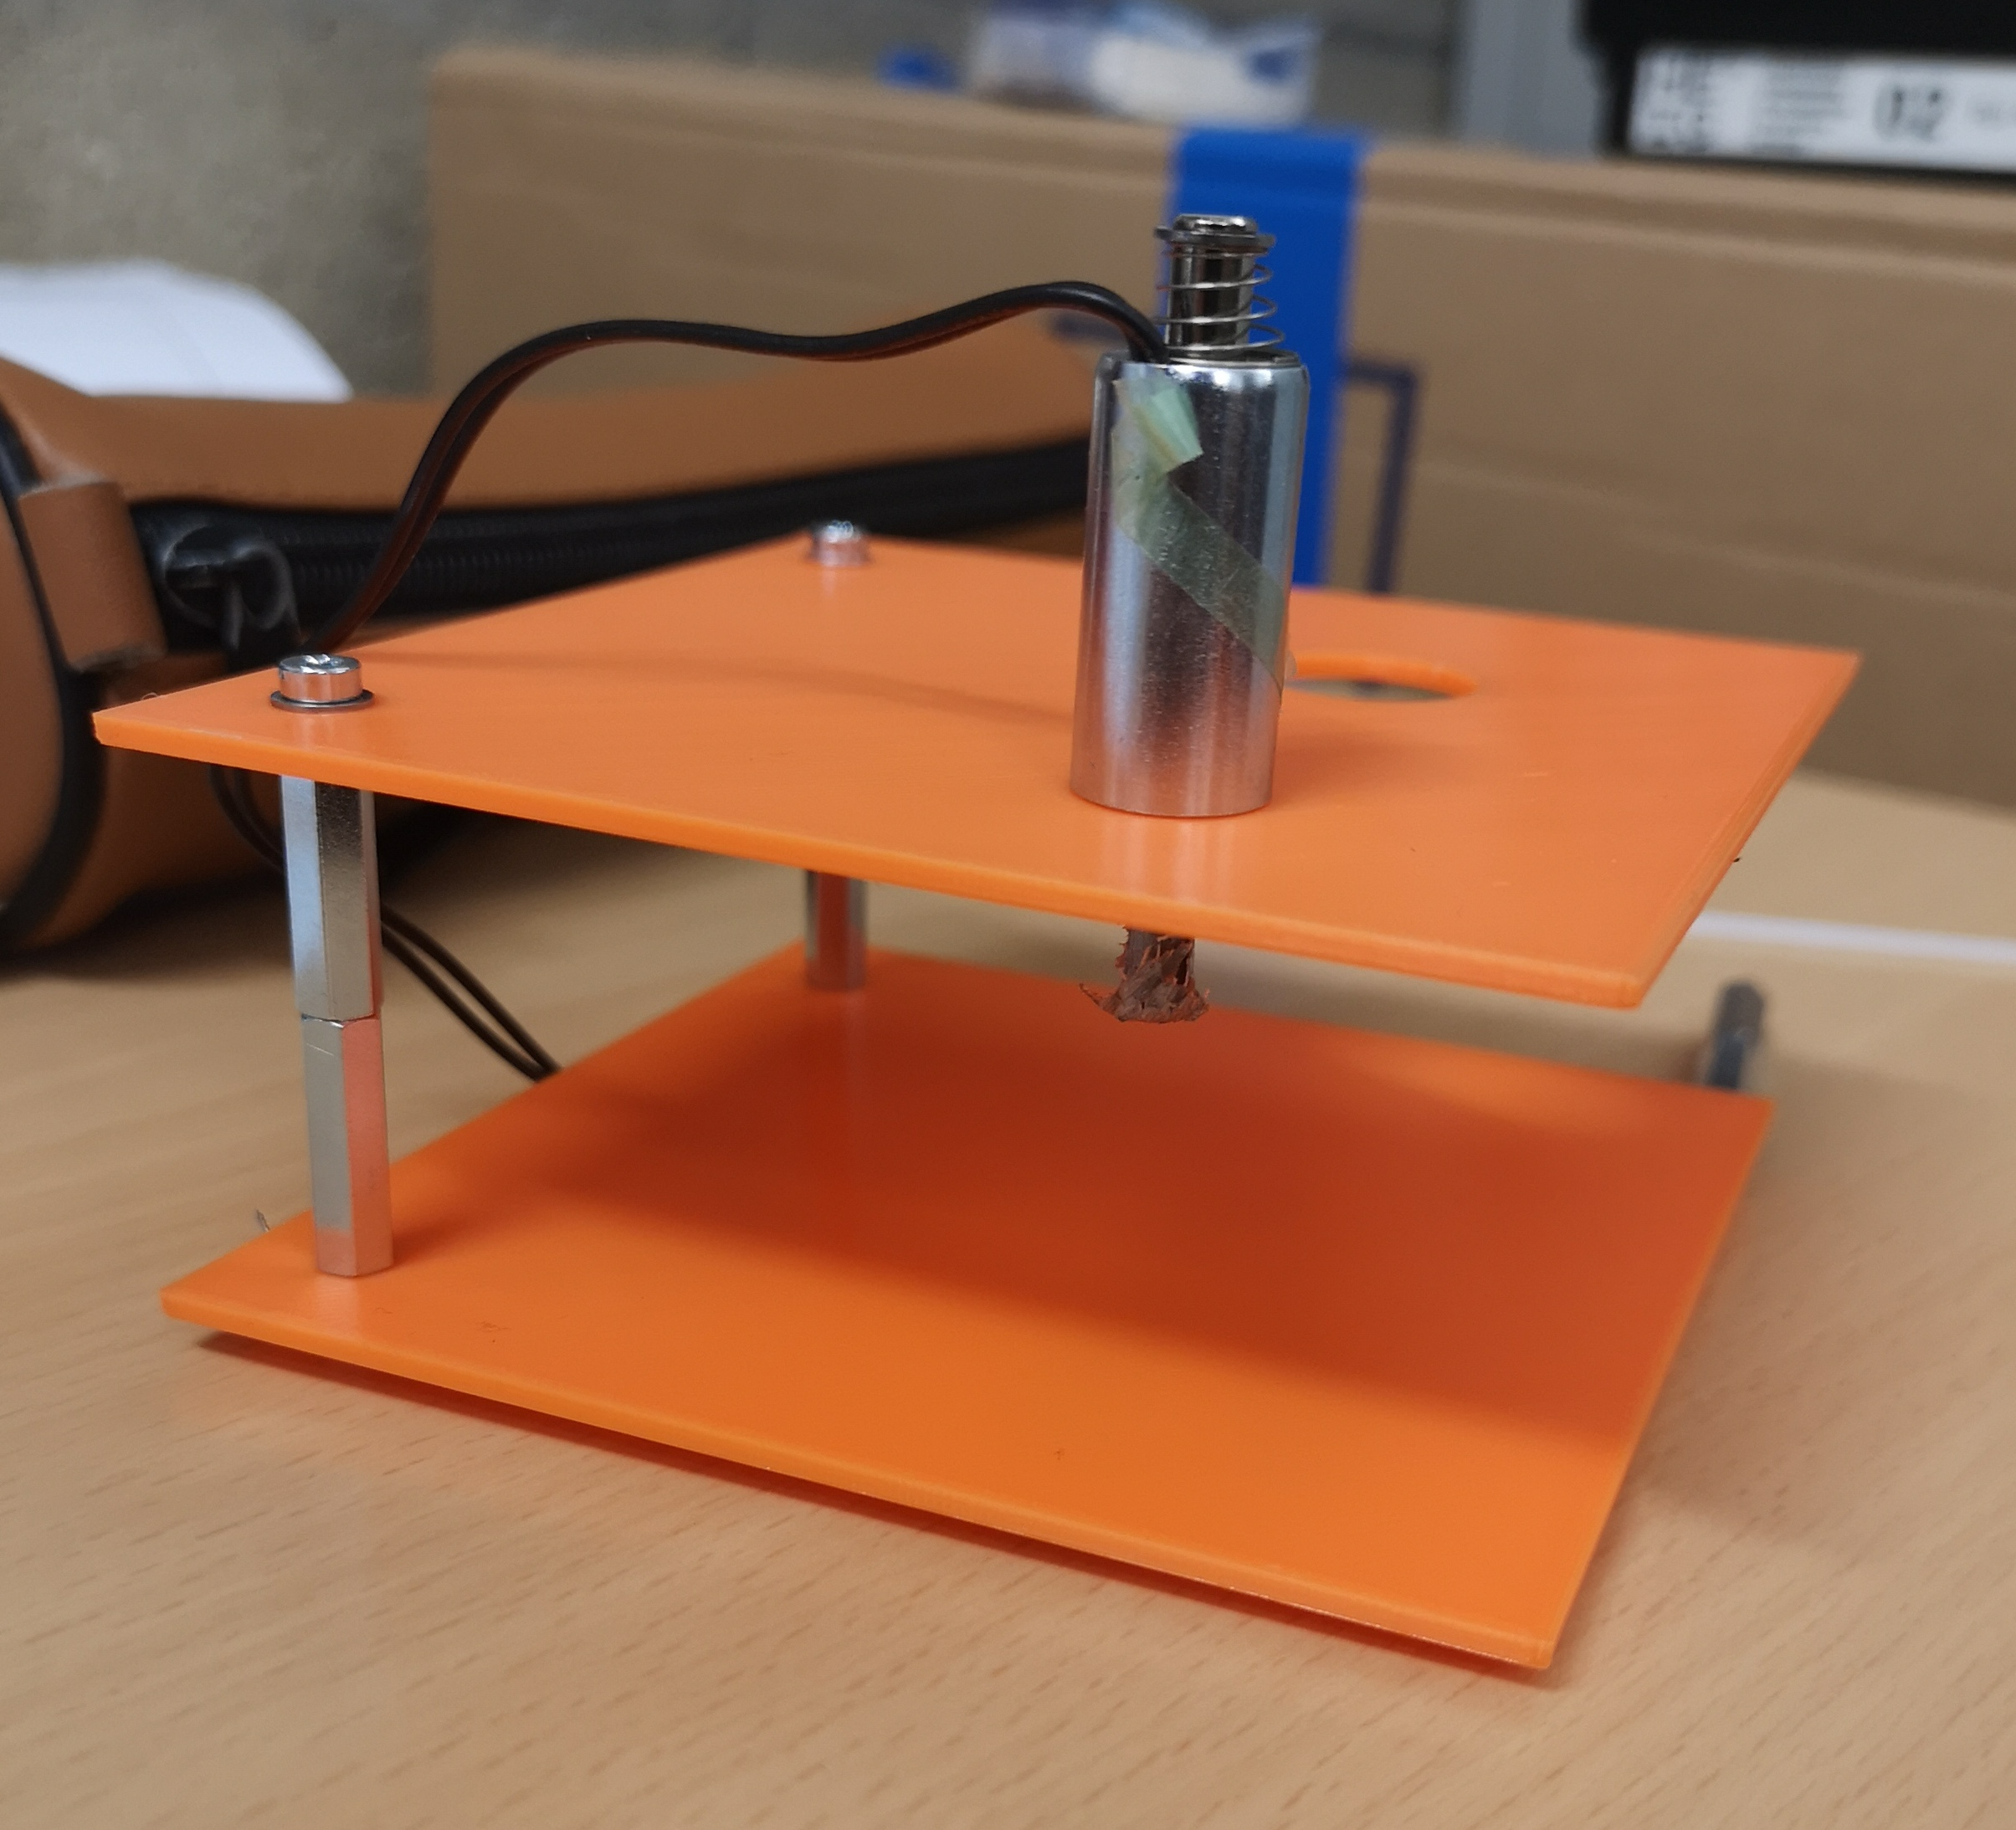
\includegraphics[width=10cm]{assets/figures/support_test_prehenseur.jpg}
    \caption{Système de préhension - Support de test}
\end{figure}

\begin{table}[h]
    \begin{center}
        \caption{Résultats du test de préhension}
        \begin{tabular}{|c|l|}
            Eléments       & Préhension réussite \\ \hline
            Préhenseur 11N & NON                 \\
        \end{tabular}
    \end{center}
\end{table}

Le préhenseur testé n'a pas assez de force pour presser sur les boutons de la télécommande. Il existe des modèles plus puissant, mais également
plus large, ceux-ci ne pourraient pas être placés côte-à-côte. Plusieurs autres solutions ont été présentées lors du choix du matériel, mais malheureusement
n'ont pas encore été testée.

N'ayant pas encore les caractéristiques de l'élément de préhension, l'installation du tiroir de la télécommande n'a pas été défini.

\section{Mesure de la vitesse}
Après que les traces d'hydrocarbures aient été détectées sur la route, il faut savoir quand ouvrir la section du semoir au bon moment. La distance entre la zone de détection et le semoir étant connue,
il est nécessaire de mesurer la vitesse afin de déterminer le temps après lequel il faut agir sur les ouvertures.
\subsection{Concept de mesure de vitesse}
Plusieurs solutions ont été envisagées:

\begin{itemize}
    \item Mesure par vision: L'idée serait d'utiliser l'image captée par la caméra et de la comparer avec l'image suivante. Sachant le temps entre deux images,
          la différence de position serait déterminer avec une corrélation. \underline{L'avantage} premier est que j'ai déjà la caméra, il n'y aurait pas besoin d'ajouter d'autres composants.
          \underline{Les inconvénients} sont les suivants, le filtre limitant les rayonnements visibles pourrait être problématique pour faire des corrélations, de plus, le temps de calcul nécessaire
          à une corrélation est trop grand, ce serait trop difficile de concilier efficacité de la cadence de traitement et mesure de la vitesse.
    \item Mesure par radar Doppler: Le radar Doppler permet de mesurer la vitesse relative entre deux éléments, entre un élément immobile et un véhicule par exemple. Dans notre cas d'utilisation, cette méthode n'est pas adaptée car il n'y
          a pas d'élément immobile à observer avec le radar lorsque le véhicule se déplace.
    \item Mesure par capteur à effet Hall. L'idée est de fixer un aimant sur l'essieu d'une des roues de la remorques.
          Ainsi, lorsque la roue est en mouvement, l'aimant passe devant le capteur. Sachant les dimensions du pneus de la remorque, il serait possible de déterminer la vitesse en fonction de la fréquence d'activation du capteur.
          \underline{Avantages :} Peu coûteux, facile à mettre en place, nécessite seulement de configurer une routine d'interruption sur le \Gls{rpi4}.
          \underline{L'inconvénient} majeur est la difficulté à installer le tout, de plus, les capteurs disponibles à l'école fonctionnent en 5V, or les pins I/O du Rpi4 fonctionne en 3.3V et ne tolèrent absolument pas le 5V.
    \item Mesure par capteur Reed: Le principe est identique au capteur à effet Hall, mais le fonctionnement du composant est un peu différent. Un capteur Reed est un simple interrupteur qui se ferme lorsqu'il est actionné par un aimant,
          ainsi, il est possible d'avoir du 3.3V sur les pins I/O du Rpi4.
\end{itemize}
\textbf{La mesure de la vitesse se fera par capteur Reed.}
\subsection{Programme de mesure de vitesse}
Le signal reçu depuis le capteur Reed sera un signal carré dans l'espacement entre deux flancs montant permettra de déterminer la vitesse. La mesure de celle-ci
se basera sur une routine d'interruption \cite{ed_raspberry_2020}. Les fonctions concernant la mesure de vitesse se trouvent aussi dans le fichier \underline{detection\_lib.py}.
\begin{itemize}
    \item speed\_calculation\_callback(channel), callback d'interruption mesurant le temps entre chaque appelle et calculant la vitesse.
    \item get\_speed(), fonction getter qui retourne la vitesse calculée par le callback.
\end{itemize}


Dans un premier temps, le fonctionnement du code a été vérifié en utilisant un générateur de signaux, paramétré de manière à avoir un signal carré de 3.3V d'amplitude.
J'ai défini dans le code que le diamètre de la roue du semoir est de 0.7 [m], voici les résultats:

\begin{table}[h]
    \begin{center}
        \caption{Mesure de vitesse par génération de signaux}
        \begin{tabular}{|c|c|c|c|}
            Fréquence [Hz] & Vitesse théorique [m/s] & Vitesse retourné [m/s] & Différence  [\%] \\ \hline
            1              & 2.199                   & 2.199                  & 0                \\
            0.5            & 1.099                   & 1.099                  & 0                \\
        \end{tabular}
    \end{center}

    A noter que dans ce cas, la vitesse en fonction de la fréquence se calcul de la manière suivante: \(V = D / t = diam*pi*freq\)
\end{table}

Les résultats étant bon, dans un deuxième temps, j'ai testé la mesure de vitesse avec le capteur Reed. Pour simuler la rotation de l'essieu en laboratoire,
l'assemblage suivant a été effectué:

\begin{figure}[H]
    \centering
    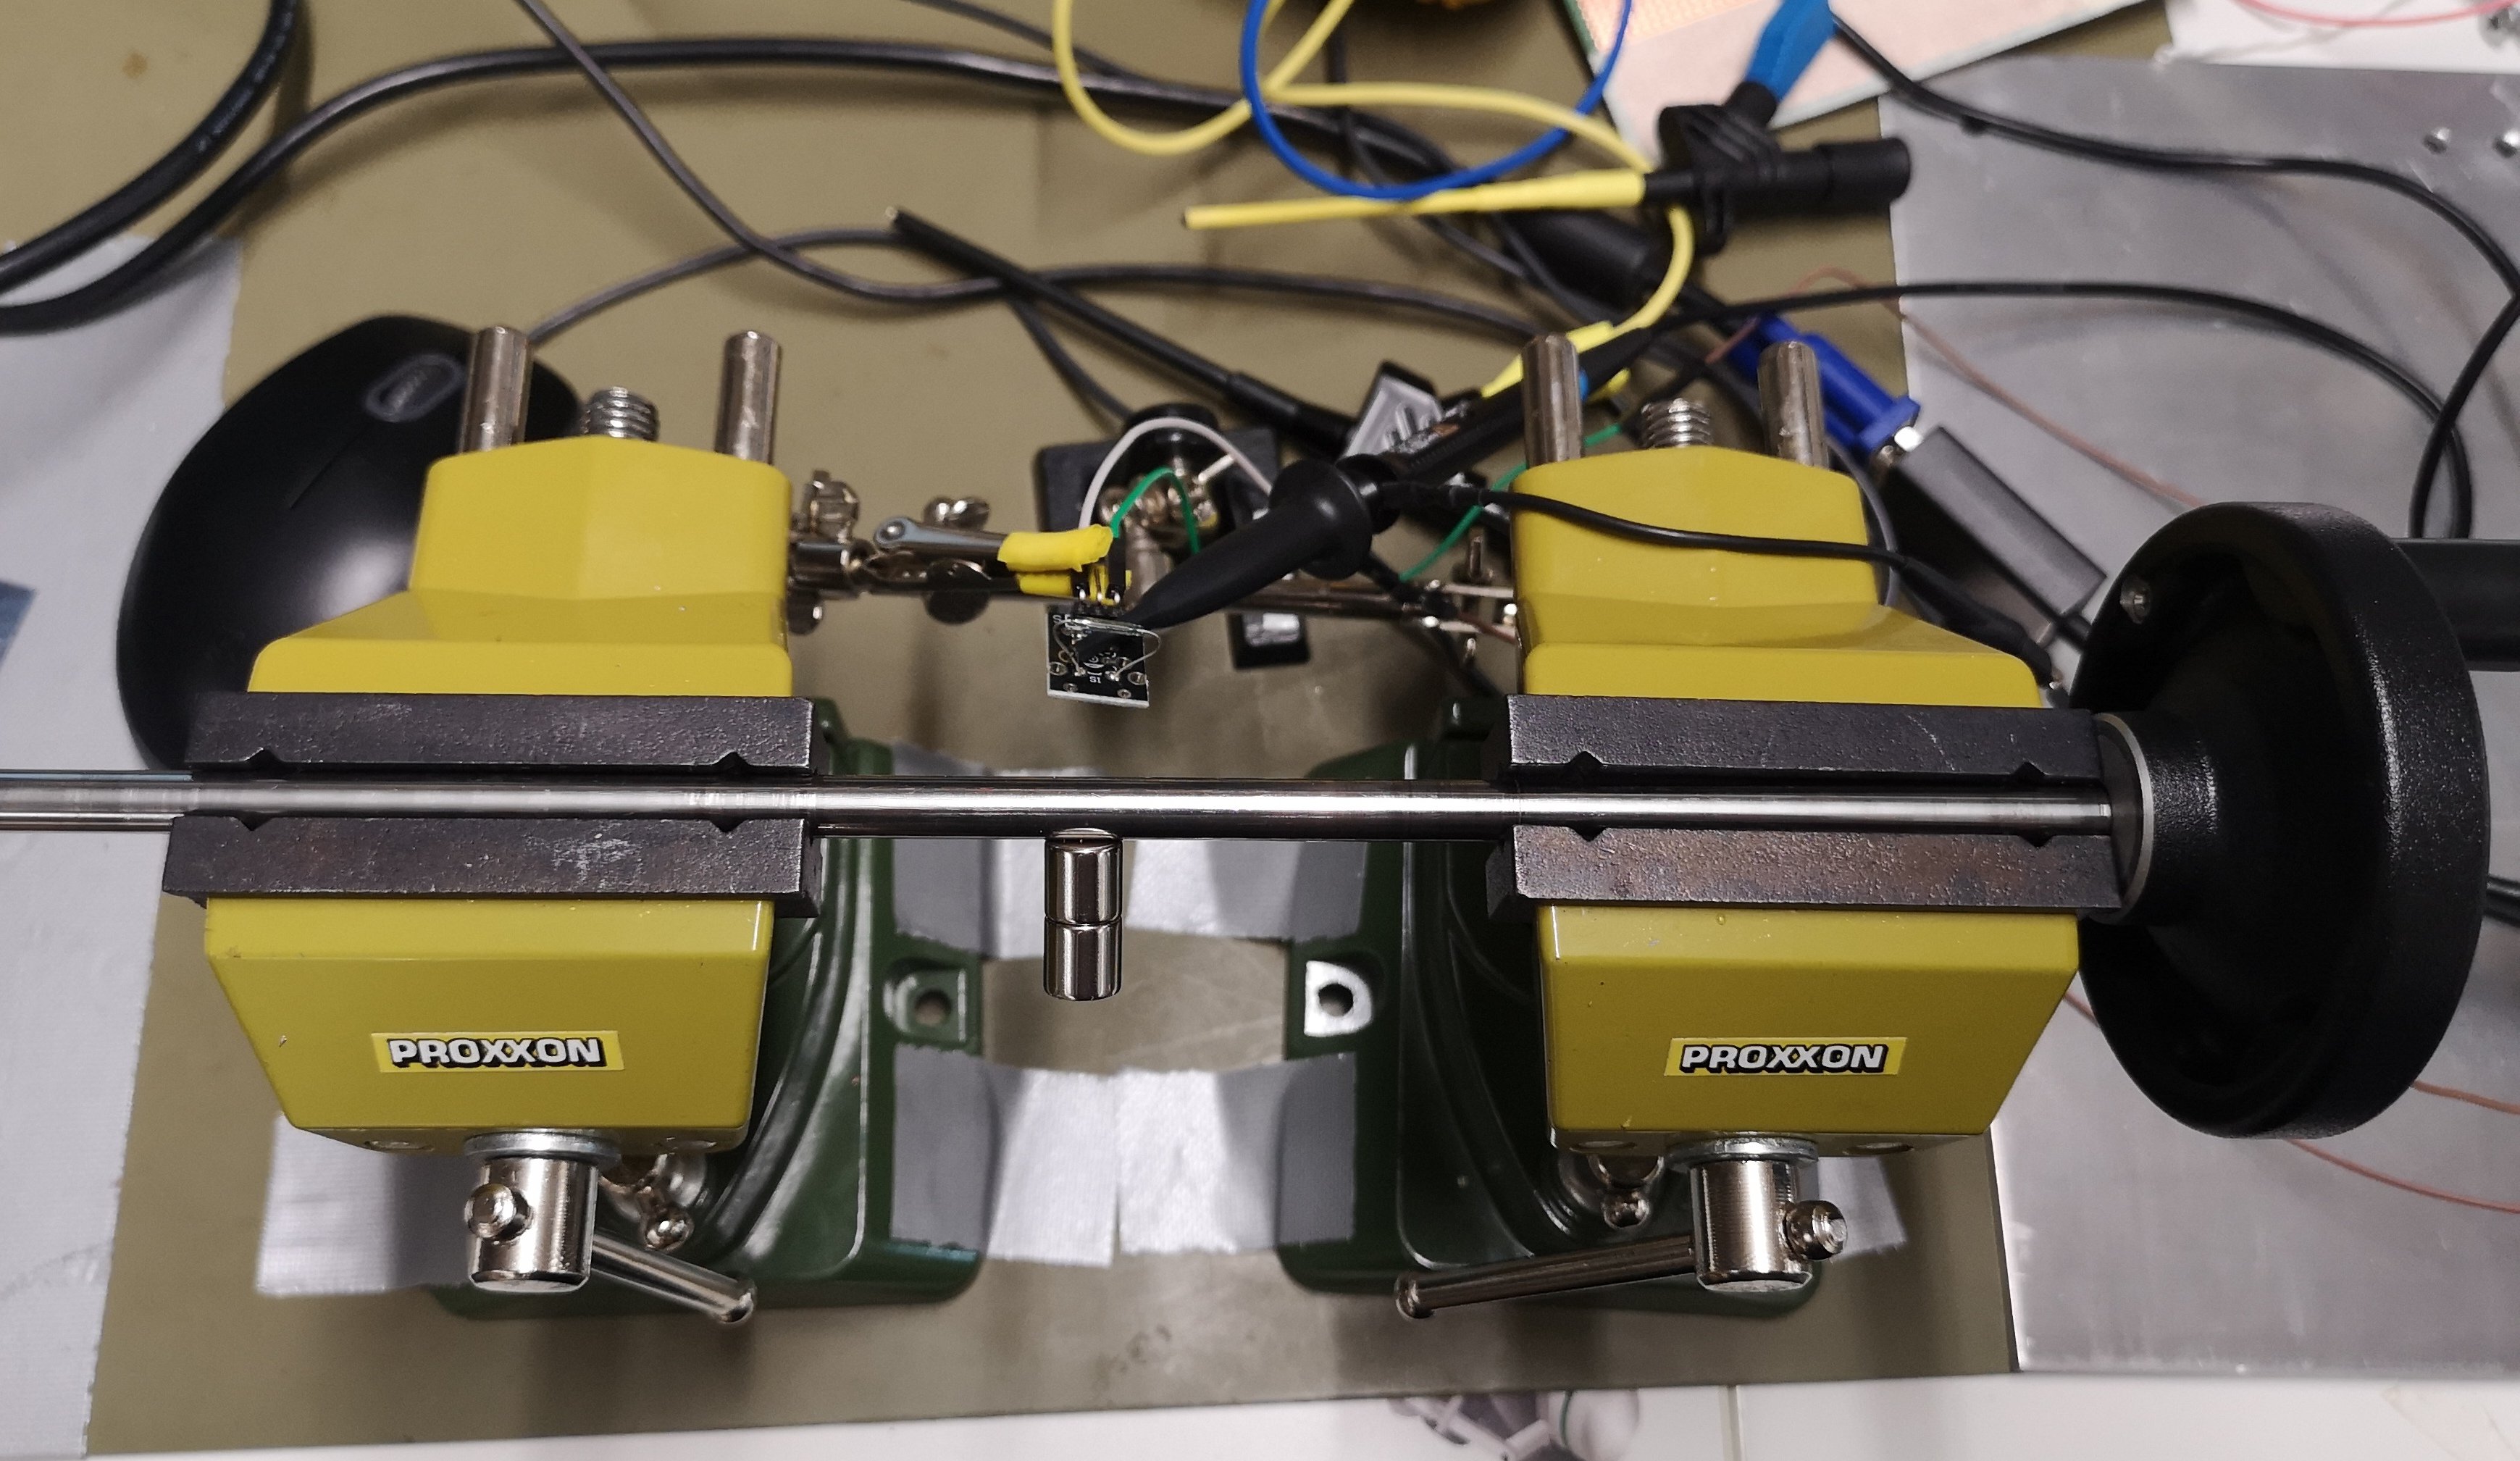
\includegraphics[width=12cm]{assets/figures/essieu.jpg}
    \caption{Mesure de vitesse - Montage de test}
\end{figure}
Un aimant est accroché à la barre, la manivelle permet de faire tourner la barre, faisant passer l'aimant devant le capteur.
Notons que ce capteur Reed et les aimants ont été trouvés au \gls{fablab} et leurs caractéristiques ne sont pas connues. La distance les
séparant a été déterminée en faisant des essais.

En faisant tourner l'aimant, l'Oscillogramme suivant a été observé:
\begin{figure}[H]
    \centering
    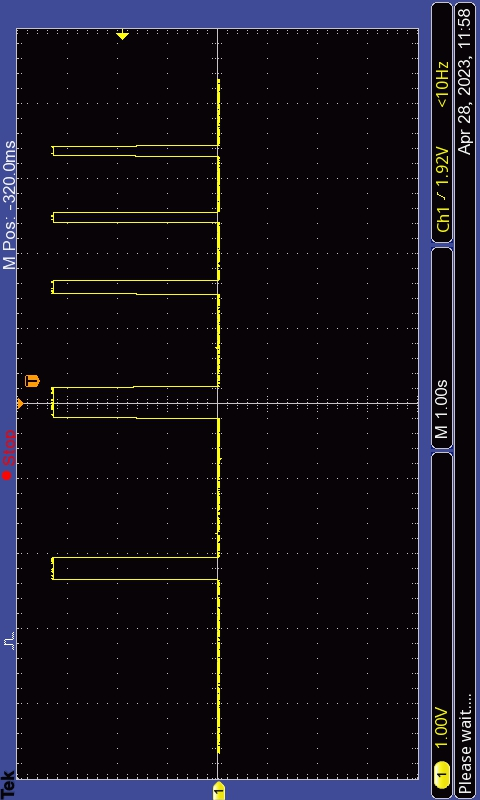
\includegraphics[width=8cm, angle=-90]{assets/figures/trame_comp.JPG}
    \caption{Mesure de vitesse - Oscillogramme}
\end{figure}

Il y a 5 flancs montant, donc 4 résultats à déterminer.

Les résultats du soft sont les suivants:
\begin{figure}[H]
    \centering
    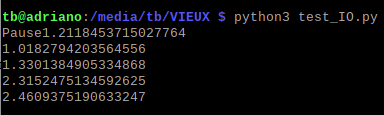
\includegraphics[width=8cm]{assets/figures/vitesse_res.png}
    \caption{Mesure de vitesse - Résultats du soft}
\end{figure}

La différence de temps entre chaque flancs montant ont été mesuré à l'aide des curseurs.
La vitesse se calcul de la manière suivante: \(V = diam*pi/$\Delta$t \)

Le pourcentage de différence: \(diff = 100*|theo-mes|/theo \)
\begin{table}[h]
    \begin{center}
        \caption{Mesure de vitesse par interruptions}
        \begin{tabular}{|c|c|c|c|}
            $\Delta$t [s] & Vitesse théorique [m/s] & Vitesse retourné [m/s] & Différence  [\%] \\ \hline
            2.16          & 1.018                   & 1.018                  & 0                \\
            1.66          & 1.324                   & 1.33                   & 0.45             \\
            0.94          & 2.339                   & 2.315                  & 1.02             \\
            0.9           & 2.443                   & 2.46                   & 0.69             \\
        \end{tabular}
    \end{center}
\end{table}

Notons que la précision du $\Delta$t dépend de la résolution de l'oscilloscope, il est donc possible que la vitesse retournée par le Rpi4
soit plus juste que la valeur théorique à laquelle elle est comparée.

L'ensemble des mesures effectuées sur la mesure de vitesse indique que la méthode est fiable. Il ne reste plus qu'à installer l'aimant sur le véritable
essieu du semoir et fabriquer un support pour que le capteur Reed soit proche de l'aimant.
\section{Programme de pilotage des vérins}
\subsection{Diagramme de fonctionnement}
Le code gérant les vérins se base sur le threading. A chaque fois qu'une donnée d'ouverture/fermeture est retournée par le traitement d'image,
un thread est ouvert et exécute le code représenté par le diagramme ci-dessous. L'exécution dépendant de la vitesse, il n'y a pas de point de synchronisation
dans le programme principal, et donc pas d'attente active.

\begin{figure}[H]
    \centering
    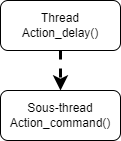
\includegraphics[height=3cm]{assets/figures/diag_command.png}
    \caption{Diagramme du script de commande}
\end{figure}

Les blocs du diagramme ci-dessus représentent des fonctions de la librairie du fichier \underline{detection\_lib.py}, respectivement:
\begin{itemize}
    \item action\_delay(distance, speed, opening\_state), cette fonction calcule le taux d'ouverture ou fermeture à appliquer aux vérins en fonction de leurs états précédents,
          attend une durée définie par la vitesse et la distance entre le champ de vision et les vérins, puis trois sous-thread de la fonction action\_command().
    \item action\_command(opening\_id, opening\_pct), cette fonction gère l'activation des préhenseurs sur la télécommande. On considère un temps défini permettant d'ouvrir un fermer à 100\% les vérins.
          puis on active les préhenseurs en fonction de ce temps. Par exemple une ouverture de 50\% du vérins prendra 50\% du temps d'ouverture maximal.
\end{itemize}
En l'état actuel, la fonction action\_delay(..) défini son temps d'attente avec ses paramètres et donc lors de l'appel. Ca signifie qu'une forte accélération provoquera un décalage avec l'actionnement des vérins.
\subsection{Test du script}
Les préhenseurs n'ayant pas été sélectionnés, les fonctions précédemment décrites ont été testée avec des inputs connues, les résultats ont été mesurés
à l'aide d'un oscilloscope.
\newpage
Ci-dessous, un relevé d'oscilloscope comprenant deux traces. \textbf{En jaune}, le signal d'une première sortie, celle-ci doit s'ouvrir à 20\% puis à 25\%,
le signal doit donc indiqué un premier état haut de 20\% du temps maximal d'ouverture, puis un second était haut de 5\% du temps maximal d'ouverture.
\textbf{En bleu}, le signal d'une seconde sortie, celle-ci doit s'ouvrir à 10\% puis à 50\%, les deux états haut doivent durer respectivement 10\% puis 40\% du temps maximal d'ouverture.

Dans le cadre de ce test, le temps maximal d'ouverture a été défini à 0.5 [s].
\begin{figure}[H]
    \centering
    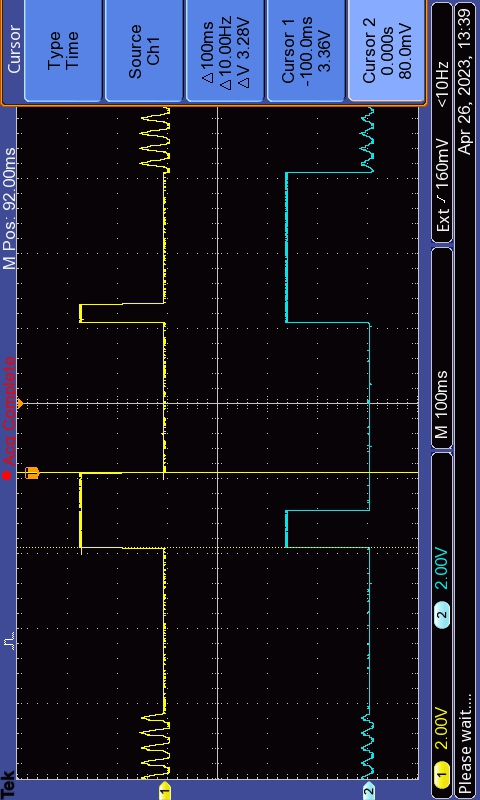
\includegraphics[width=8cm, angle=-90]{assets/figures/oscillo_commande.JPG}
    \caption{Commande - Résultats du soft}
\end{figure}

Le pourcentage de différence: \(diff = 100*|theo-mes|/theo \)
Le $\Delta$t théorique s'obtient avec \($\Delta$t = t\_max * pct\_diff\)

Les valeurs retournées ont été mesurées avec les curseurs de l'oscilloscope.
\begin{table}[h]
    \begin{center}
        \caption{Commande - Tableau de résultat du soft}
        \begin{tabular}{|c|c|c|c|}
            Inputs [\%] & $\Delta$t théorique [ms] & $\Delta$t retourné [ms] & Différence  [\%] \\ \hline
            20          & 100                      & 100                     & 0                \\
            25          & 25                       & 24                      & 4                \\
            10          & 50                       & 48                      & 4                \\
            50          & 200                      & 200                     & 0                \\
        \end{tabular}
    \end{center}
    Notons qu'avec la résolution de temps de l'oscilloscope lors de la mesure, les curseurs offrent une résolution de $\pm$ 1 [ms],
    ceci peut expliquer les différences pour les 2èmes et 3èmes résultats (qui sont d'ailleurs les états haut avec les temps les plus courts).
\end{table}

Les résultats des fonctions de commande des ouvertures et fermeture des vérins sont bons.
\newpage
\section{Câblage - Attribution des pins I/O}
Lors des tests fonctionnels du chapitre précédent, des pins ont été attribuées aux différentes entrées et sorties. Il existe deux numérotations différentes \cite{pinning_Rpi4},
le numéro d'E/S et son emplacement physique. Le câblage a été fait selon le tableau ci-dessous, des petites étiquettes avec des abréviations ont été ajoutée au montage pour éviter les confusions durant les mesures.


\begin{table}[h]
    \begin{center}
        \caption{Tableau de câblage du Raspberry Pi 4}
        \begin{tabular}{|c|c|c|c|}
            Type de E/S             & Abréviations & Pin GPIO & Pin header \\ \hline
            3.3[V]                  & 3.3[V]       & -        & 1          \\
            Masse                   & Masse        & -        & 6          \\
            Vérins gauche ouverture & L\_on        & 17       & 11         \\
            Vérins gauche fermeture & L\_off       & 18       & 12         \\
            Vérins centre ouverture & C\_on        & 19       & 35         \\
            Vérins centre fermeture & C\_off       & 20       & 38         \\
            Vérins droite ouverture & R\_on        & 21       & 40         \\
            Vérins droite fermeture & R\_off       & 22       & 15         \\
            Mesure de vitesse       & Inter        & 16       & 36         \\
        \end{tabular}
    \end{center}
\end{table}